\documentclass[11pt]{article}\usepackage[]{graphicx}\usepackage[]{color}
%% maxwidth is the original width if it is less than linewidth
%% otherwise use linewidth (to make sure the graphics do not exceed the margin)
\makeatletter
\def\maxwidth{ %
  \ifdim\Gin@nat@width>\linewidth
    \linewidth
  \else
    \Gin@nat@width
  \fi
}
\makeatother

\definecolor{fgcolor}{rgb}{0.345, 0.345, 0.345}
\newcommand{\hlnum}[1]{\textcolor[rgb]{0.686,0.059,0.569}{#1}}%
\newcommand{\hlstr}[1]{\textcolor[rgb]{0.192,0.494,0.8}{#1}}%
\newcommand{\hlcom}[1]{\textcolor[rgb]{0.678,0.584,0.686}{\textit{#1}}}%
\newcommand{\hlopt}[1]{\textcolor[rgb]{0,0,0}{#1}}%
\newcommand{\hlstd}[1]{\textcolor[rgb]{0.345,0.345,0.345}{#1}}%
\newcommand{\hlkwa}[1]{\textcolor[rgb]{0.161,0.373,0.58}{\textbf{#1}}}%
\newcommand{\hlkwb}[1]{\textcolor[rgb]{0.69,0.353,0.396}{#1}}%
\newcommand{\hlkwc}[1]{\textcolor[rgb]{0.333,0.667,0.333}{#1}}%
\newcommand{\hlkwd}[1]{\textcolor[rgb]{0.737,0.353,0.396}{\textbf{#1}}}%

\usepackage{framed}
\makeatletter
\newenvironment{kframe}{%
 \def\at@end@of@kframe{}%
 \ifinner\ifhmode%
  \def\at@end@of@kframe{\end{minipage}}%
  \begin{minipage}{\columnwidth}%
 \fi\fi%
 \def\FrameCommand##1{\hskip\@totalleftmargin \hskip-\fboxsep
 \colorbox{shadecolor}{##1}\hskip-\fboxsep
     % There is no \\@totalrightmargin, so:
     \hskip-\linewidth \hskip-\@totalleftmargin \hskip\columnwidth}%
 \MakeFramed {\advance\hsize-\width
   \@totalleftmargin\z@ \linewidth\hsize
   \@setminipage}}%
 {\par\unskip\endMakeFramed%
 \at@end@of@kframe}
\makeatother

\definecolor{shadecolor}{rgb}{.97, .97, .97}
\definecolor{messagecolor}{rgb}{0, 0, 0}
\definecolor{warningcolor}{rgb}{1, 0, 1}
\definecolor{errorcolor}{rgb}{1, 0, 0}
\newenvironment{knitrout}{}{} % an empty environment to be redefined in TeX

\usepackage{alltt}

\usepackage{hyperref, lastpage, fancyhdr}
\usepackage{amsmath}
\usepackage{float}



\topmargin      -1.5cm   % read Lamport p.163
\oddsidemargin  -0.04cm  % read Lamport p.163
\evensidemargin -0.04cm  % same as oddsidemargin but for left-hand pages
\textwidth      16.59cm
\textheight     23.94cm
\parskip         7.2pt   % sets spacing between paragraphs
\parindent         0pt   % sets leading space for paragraphs
\pagestyle{empty}        % Uncomment if don't want page numbers
\pagestyle{fancyplain}

\usepackage{natbib} %need this for bibtex
\IfFileExists{upquote.sty}{\usepackage{upquote}}{}

\lhead{}
\chead{}
\rhead{}

\usepackage{setspace} %for double spacing
\doublespacing
\IfFileExists{upquote.sty}{\usepackage{upquote}}{}
\begin{document}




\title{Measuring Energy Intake via Energy Balance Equation while Accounting for Measurement Error}
\author{Daniel Ries}
\date{\today}
\maketitle


%---------------------------------------------------------------------------------------------------------%
\section{Introduction}
%-----------------------------------------------------------------------------------------------------------%

Accurately measuring one's energy intake (EI measured in kcals consumed) is a very difficult task \cite{cook},\cite{johnsonr},\cite{jakes}. This is especially true for measuring energy intake in free living conditions and not in inpatient, controlled settings \cite{martin}. It has been said that our inability to measure energy intake accurately is the one of  the biggest pitfalls of obesity research \cite{winkler}, \cite{gilmore}. According to the National Institute of Diabetes and Digestive and Kidney Diseases, 66.8\% of adults in the US are overweight or obese, and 35.7\% are obese \cite{niddk}. Obesity has been linked to a multitude of negative health effects like cardiovascular disease \cite{wilson}, high blood pressure, Type 2 diabetes, some cancers, stroke, osteoarthritis, and mental illness \cite{cdc}, \cite{kasen}, \cite{luppino}. It has been found that the number of chronic conditions due to obesity is larger than that of smoking or drinking \cite{sturm}. Because of this, obesity has been a hot topic in legislation and the health care industry. Being able to accurately measure energy intake would be extremely useful to monitor patient compliance with set diets \cite{hall11}. The so called \emph{6 month plateau}, which is the typical flattening of weight loss seen by those on weight loss programs after 6 months, has recently been attributed to noncompliance rather than metabolic adaptation \cite{hall10}, \cite{thomas14}. This is important because validated models show this weight loss should continue for between one and two years. This is an issue because the patients still report diet adherence \cite{thomas14}. It has been argued that mathematical modeling could help in assessment of adherence in diet interventions \cite{brady14}, \cite{thomas13}.  Dynamic mathematical models to predict an individual's energy intake have started to gain attention, partly due to the now widespread knowledge that Wishnofsky's assertion that one pound of body mass is equivalent to 3500 calories \cite{thomas14b} is false. These models have shown the benefits of collaboration across multiple disciplines by advancing the field of obesity research greatly. However, these models use as an input data that is measured with error. In this dissertation, we develop statistical methods to assess the extent of measurement error and bias and calibrate the noisy measurements that in turn will make these new mathematical models even more useful. 

In this chapter we review methods for measuring EI and after introducing the energy balance principle, methods for measuring energy expenditure (EE) and changes in energy stores $\Delta$ES. We then discuss modeling energy balance as a whole. We then explore statistical methods for analyzing data with measurement error. \\

%--------------------------------------
\subsection{Measurement Instruments}
%----------------------------------------

%-----------------------------------%
\subsubsection{Measuring Energy Intake}
%-----------------------------------%

There are several ways one can estimate the energy intake of a free living human. One of the more common methods, a self-report via a food frequency questionnaire (FFQ), is known to be biased and an unreliable measure \cite{schoeller}, \cite{freedman},\cite{schaefer00}. This method, however, continues to be popular due to its low cost and ease to implement on a large sample. A FFQ is a checklist that asks one to mark how many times one ate a specified food during a specified period of time. Portion size may or may not be collected. 24 hour recalls are another popular option \cite{rjohnson}. These are typically conducted over the phone or sometimes in person. A trained dietician using administers these recalls. These are popular because they are relatively cheap compared to other methods, and they only require remembering 24 hours of food consumption. Additionally, if the recalls are done randomly, then the diets of individuals being surveyed are not affected. However, there still remains a considerable amount of within person variability unless many 24 hour recalls are taken on the same individual. This is also still a form of self report meaning individuals can lie about what they ate or forget, although the multiple pass method helps aleviate this issue \cite{raper}. Doubly labeled water (DLW) has been called the gold standard for estimating energy intake when individuals are weight stable \cite{gilmore}, \cite{hall11}, \cite{thomas11a}. Patients drink a small amount of liquid that contains an isotope of hydrogen and oxygen. Two weeks later a urine sample is taken and the concentrations are measured to get an estimate of energy expenditure that is estimated based on washout kinetics \cite{thomas11a}. However, we are not only interested in weight stable individuals, but also those who are gaining and losing weight as well. Moreover, DLW is expensive and requires trained personnel to administer and analyze, therefore it is not reasonable to give DLW to all study participants \cite{hall14}, \cite{thomas11a}. DLW has found to have an average error of between 2-8\%, which depends on the loading dose, length of metabolic period and number of samples \cite{schoeller88}. Direct calorimetery is based on production of heat by a human, and it provides accurate estimates of energy expenditure, but it must be administered in a special lab setting, and the patient must be in energy balance \cite{laporte85}. Indirect calorimetry is similar, except the patient has a mask that collects the air exhaled and gives an accurate measure of energy expenditure, but like direct calorimety,  the patient must be in energy balance for this to give a measure of energy intake \cite{laporte85}. Neither of these options provide realistic measures if we are talking about free living humans because clearly, these instruments would affect one's everyday life. Several other new methods of measuring energy intake accurately and cheaply have been proposed: food photography \cite{daugherty12}, bite count devices \cite{fontana15}, and devices that measure chewing \cite{scisco13}, however, for obvious reasons such as influencing food intake, these methods still don't meet the need for an accurate, noninvasive, and relatively cheap measure of energy intake \cite{sanghvi15}.


%------------------------------------------%
\subsubsection{Energy Balance Principle}
%------------------------------------------%

Another approach to measuring EI that has gained popularity more recently is through what's called the energy balance principle. The energy balance equation is given in (\ref{eb}). This principle is based off of the \emph{first law of thermodynamics}, that is,  energy can neither be created or destroyed. Looking at (\ref{eb}), it is easy to see that we can rewrite EI as a simple function of energy expenditure (EE) and the change in energy storage ($\Delta$ES). In other words, instead of trying to measure energy intake directly via the methods of the previous section (which were either notoriously inaccurate, or unreasonably expensive), we can try to measure EE and $\Delta$ES and calculate EI. The energy balance model has been found to be an accurate and precise assessment of EI, at least during weight gain \cite{gilmore}. Many models have shown up in the epidemiology and nutrition journals using this approach \cite{hall10}, \cite{thomas11a}, \cite{thomas10}, \cite{sanghvi15},\cite{hall11}, \cite{racette11}. Although it may seem like we are complicating the problem by having to estimate two quantities instead of one, it turns out EE and $\Delta$ES are easier to measure accurately and cheaply.




\begin{align}
  \Delta \text{ES} &= \text{EI - EE}
  \label{eb}
\end{align}

%------------------------------------------%
\subsubsection{Measuring Energy Expenditure}
%------------------------------------------%

From (\ref{eb}), if we want to estimate the EI for an individual, we need to have estimates for both EE and $\Delta$ES. We will focus on EE in this section, and $\Delta$ES in the next section. We refer to EE as the amount of energy used by an individual in a day, measured in kcals. There are a number of different ways our bodies burn calories, so we can break EE into four components:dietary induced thermogensis (DIT), volitional physical activity (PA), resting metabolic rate (RMR), and spontaneous physical activity (SPA) \cite{thomas11a}. 

\begin{align}
  \text{EE} &= \text{DIT + PA + RMR + SPA}
	\label{ee}
\end{align}

DIT is related to the energy used when digesting, metabolizing, and transporting food \cite{thomas11a}. If one eats more food, then his or her body must use more energy to process that food and vice versa. Thomas et al. assumes that DIT is proportional to EI and thus is estimated by a single value $\beta$. PA represents all fitness related activities such as walking, running, playing sports, etc \cite{thomas11a}. We refer to these as voluntary activity, as one could technically live without burning calories this way. Thomas et al. measures PA as being proportional to body mass. RMR is the energy expended in order to keep the body functioning \cite{thomas11a}. Thomas et al. uses the Livingston-Kohlstadt equation to calculate RMR. SPA is the energy used through changes in posture and fidgeting \cite{thomas11a}. Thomas et al. notes that measuring SPA is very difficult, but use that the ratio of change in SPA to change in  EE is constant. Thus, they use an integration along with the relationship in (\ref{ee}) to get an estimate. \\

The beauty of many of the EE measurement methods is that we don't need to measure each of those four components separately. We already discussed one of the available methods for measuring EE in the previous section. DLW is considered the gold standard measurement for EE \cite{lagerros},\cite{bouten},\cite{thomas11},\cite{hall11},\cite{gilmore},\cite{sanghvi15}, \cite{racette11}, and it provides an estimate of EI if an individual is weight stable, otherwise by (\ref{eb}) it doesn't tell the whole story. As discussed before DLW does give us the best estimate but at a very high cost. Alternatives to DLW to measure EE exist. Consumer based physical activity monitors with accelerometers have become popular in recent years. Products such as Fitbit, Nike Fuel Band, Jawbone UP band, and Basis B1 Band that measure steps taken, calories burned, heart rate, sleep, GPS, etc. are available to the general public at reasonable cost. They have become more popular in the research area as providing a measure of EE \cite{welk04}, and their reliability has been tested \cite{bassett00},\cite{drenowatz11},\cite{johannsen10},\cite{dannecker13},\cite{lee}. The results are promising, the physical activity monitors seem to give a relatively cheap, accurate, and objective measure of EE. \\

The SenseWear Pro3 armband (SWA) and SenseWear Mini (mini) specifically have been shown to be relatively good measures of energy expenditure \cite{johannsen10}. The SWA has a biaxial accelerometer while the mini has a triaxial accelerometer. Some of what makes these standard apart from popular alternatives like Fitbit, is they also have sensors to measure heat flux, temperature, and galvanic skin response. One of the concerns with these wearables is assessing compliance. It is often hard to tell if someone has been following the researcher's directions of using the device. The SWA and mini don't have this problem as they provide estimates of wear time directly \cite{johannsen10}. These two specific devices are not without flaws though, as both tend to underestimate EE from more vigorous levels of activity compared to DLW. \\

Self reports are also commonly used to measure EE largely due to their ease and cost. They have the benefit of providing details in terms of type of exercise as well as duration, intensity, etc. that an activity monitor would provide. Like with EI, we have the same issue with reporting bias and are not an accurate measure of EE \cite{neilson08}. Respondents typically overestimate their activity and its intensity. However, this cheap method can provide a rough activity level estimate and allow one to categorize participants by an approximate activity level if desired. \\

Pedometers are another cheap and easy method of estimating EE. Like self-report, they contain a lot of variability. Since they only count steps, pedometers do not tell us anything about intensity or duration of exercise. This can be an issue, for instance, 3000 steps walking in a day versus 3000 steps sprinting in a day will result in the same predicted EE, when in reality, the EE would be vastly different. Like self-reports, pedometers can at least give an approximate population measure of activity. Heart rate monitors are another cheap and easy way to measure EE. Heart rate monitors provide accurate measures of heart rate, but factors other than exercise alone can affect heart rate. Temperature, emotional state, hydration status, fitness level, and age can all affect the heart rate of an individual. Direct observation is when trained personnel observe and record participant activities. This way, all activities can be monitored and objectively recorded. Of course, this method is extremely time consuming because someone must track a single participant. This can be difficult in large sample studies. These can be used to validate activity monitors, pedometers, or heart rate monitors. 




%--------------------------------------------%
\subsubsection{Energy Storage}
%-------------------------------------------%

The other term we must estimate in order to use the energy balance principle is the change in energy stores over a specified period of time. We will deal with ES in terms of relative storage, that is, the change in energy stores since the last body composition measurement. For body composition, we will deal with fat mass (FM) and fat free mass (FFM) and assume total body mass = FM + FFM. The validated equation \cite{thomas12a}  below (\ref{es}) shows how we can further break down equation (\ref{eb}).

\begin{align}
	\Delta \text{ES} &= c_{FFM} \frac{\Delta \text{FFM}}{\Delta \text{t}} + C_{FM} \frac{\Delta \text{FM}}{\Delta \text{t}}
	\label{es}
\end{align}

Where the estimates $c_{FFM}=1020$ and $c_{FM}=9500$ represent the energy densities of FFM and FM respectively. These numbers are estimates that are prone to measurement error, as in a different study, same author,  \cite{thomas10}, $c_{FFM}=1100$ and $c_{FM}=9300$ was used. \\

Setting aside the issue of measuring the energy densities of FM and FFM, we are left with the issue of measuring the change in FM and change in FFM over a specified period of time. This boils down to: how to we measure FM and FFM for an individual? Dual-energy X-ray absorptiometry (DXA) is considered the gold standard to measure fat mass (FM) and fat free mass (FFM) \cite{thomas11a},\cite{thomas11},\cite{sanghvi15},\cite{gilmore}. DXA scans are often used to measure bone mineral density, often to diagnose or track osteoporosis, but it also gives measures of body composition. As one might imagine, DXA scans are not cheap due to the specialized equipment and personnel needed. \cite{hind11} shows the precision of the new GE Lunar iDXA machine. Coefficient of variation for both FM and FFM were under 1\%.  \\


Air displacement plethysmography (ADP) is another measure of body composition. ADP measures body volume through Boyle's Law, which describes the inverse relationship between volume and pressure \cite{baracos11}. After an intial up front cost, ADP machines can be used quite easily and cheaply as no highly trained personnel is needed. It is also very quick to get a measurement and can be used for a wide variety of the population including obese and elderly. Bod Pod is one of the well known measurement tools that performs this. \\


Bioimpedance spectroscopy (BIS) also provides a relatively accurate and cheap way to measure body composition. In short, BIS instruments have sensors at one's extremities (or a subset of them), and it sends a shock at one end and measures the resistance to reach the other end(s). The results are dependent upon body water levels, which can then be a proxy for FM versus FFM . There are various different levels of quality for these machines. One can buy a cheap and easy to use one at a local nutrition store that is not particularly accurate, and much more expensive, research quality devices are also available. One of the issues with this approach is hydration levels. Since this method provides a measure of body composition that is based on how a shock passes through the body as a function of body water, one's hydration status could heavily affect the results. \\


Calipers are one of the cheapest and easiest tools to measure body composition. The caliper method takes measurements of skinfolds at certain locations to estimate \% body fat (and then can be used to calculate FM and FFM). The tool itself costs less than \$100, and someone can be quickly trained to use a caliper. Of course with this comes lots of error. \\


%-------------------------------------%
\subsubsection{Estimating Energy Intake via Energy Balance Equation}
%-------------------------------------%

Based on the availability of alternative measures of self report for EE and $\Delta$ES, we prefer to calcualte EI using the energy balance equation. To achieve the goal of measuring EI, we simply would add the estimates of EE and $\Delta$ES. However, care must still be taken, since (\ref{eb}) holds in principle, that is, if we know EE and $\Delta$ES exactly for a specified period of time, but even with DXA and DLW measurements we don't have perfect data. Thomas took this approach in her 2010 paper \cite{thomas10}, but noted that even with DXA and DLW measurements, the energy balance equation wasn't in equality, and she hypothesized this was largely due to measurement error and biological variation.

%------------------------------------------%
\subsection{Modeling Energy Balance}
%------------------------------------------%

We seek to develop a joint model for energy balance measurements that accounts for all forms of measurement error and biases. Ultimately, we would like to be able to accurately measure EI using cheaper and easier to administer devices compared to DXA and DLW. In the end, we want to calibrate these cheaper alternatives to the gold standards DXA and DLW to estimate EI. Those who have developed and tested models based on the energy balance principle have not taken measurement error into consideration, and as we've discussed, it shows up in a multitude of locations. 


Here we will give a brief introduction into what we mean by dealing with the measurement error inherent in this problem. Our ultimate objective is to estimate true EI, and of course if were able to observe this, our problem would be done. Instead, we are using the energy balance principle, and thus if we were able to observe EE and $\Delta$ES, our problem would be done as well. However, instead of observing these two quantities exactly, we gather information on EE by, for instance DLW, and $\Delta$ES by, for instance, DXA. But as we've said, these are not perfect measurements and thus have noise involved that we aim to quantify. Moreover, using DXA and DLW as a final product to estimate EI is unreasonable. We would like to measure EI accurately using cheap and easy tools like armband monitors and calipers. Armband monitors give an estimate of EE for a fixed period of time, but they are prone to even more error than DLW, and we want to measure this error. In the end, we want to calibrate the cheaper tools using our results from the measurement error model. The main benefit is future studies requiring measurements of EI, EE or $\Delta$ES would be able to use our model and calibrate cheaper tools to get data that is closer to the truth without having to use gold standard measurements.



%------------------------------------------------------------------------------------------------------------%
\subsection{Measurement Error Modeling}
%-------------------------------------------------------------------------------------------------------------%

Here we give a brief overview of measurement error modeling in statistics. We will go over basic considerations, simple models and classical methods. Then we will extend to more complicated models that are nonlinear and involve heterogeneous variance. We will examine Frequentist and Bayesian methods, and parametric, nonparametric, and semiparametric models. Complete overviews can be found in \cite{linear}, \cite{nonlinear}, \cite{buzas}.

%--------------------------------%
\subsubsection{Dangers of Ignoring Measurement Error}
%--------------------------------%

For the purposes of this report, measurement error refers to not being able to measure a covariate, or explanatory variable {\bf X} precisely. That is, instead of observing {\bf X}, we actually observe another quantity {\bf W}, that is not always (and rarely ever is) equal to {\bf X} even though our interest still lies in the relationship between the response variable {\bf Y} and the true explanatory variable with no error, {\bf X}. We still allow the possibility of observing some covariates without error, and we denote these with {\bf Z}. Recall, one of the assumptions made in linear regression using OLS is that the explanatory variables are measured without error. \\

 Data collected in the epidemiology and kinesiology fields often have measurement error due to the nature of the studies. For example, if one was trying to understand the relationship between obesity and heart disease, one would be interested in how much that person eats on average. But determining someone's average daily caloric intake is incredibly difficult, and so we could use a Food Frequency Questionnaire (FFQ). This might seem like a reasonable way to determine how much someone eats on average, that is randomly picking a week or month and have the person of interest record what they consume. The time was chosen randomly, but does a week or month really describe that person's \emph{usual} consumption patterns? The time of the year, weather, social desirability, etc. are all going to affect what the person actually eats and actually records eating. Therefore an estimate of EI based on the FFQ for \emph{usual} daily consumption is not likely going to be the true value, or sometimes not even close due to bias (see pg. 8 \cite{nonlinear}). Then this mismeasured explanatory variable will surely affect our estimated relationship between obesity and heart disease. \\


As a result, when measurement error is present in covariates, it can have a major impact on the statistical analysis performed if it is ignored. For one, it will bias estimates. This means the estimated effects will be biased in one direction or another and therefore not giving the whole story. Another problem is the loss of power in determining relationships between variables. Having measurement error in covariates essentially clouds the data with extra noise making it harder to see the true relationships and thus miss meaningful conclusions. \\


% %--------------------------------%
% \subsubsection{Differential Error}
% %---------------------------------%
% 
%  We say the error in {\bf W} with respect to {\bf X} is non-differential if {\bf Y} is conditionally independent of {\bf W}. In other words, $f_{Y|X,Z,W}=f_{Y|X,Z}$. If this doesn't hold, then we say the error is differential If the error is non-differential, {\bf W} is called a \emph{surrogate} or \emph{proxy} for {\bf X}. Clearly, assuming non-differential error can be used as a simplifying assumption, and it is often the case that this is a valid assumption. Continuing on the obesity/heart disease example above, if we knew the true average daily EI of someone, we wouldn't have reason to have them fill out a FFQ, and it probably wouldn't give us any more information about the chances of heart disease by having him/her fill one out. This would be the rational for assuming non-differential error.  The distinction is not always easy, and Buzas et al. \cite{buzas} gave a nice way to think about it: Consider whether {\bf W} would have been measured had {\bf X} been available. If it wouldn't have, non-differential error is reasonable. . 

%-----------------------------%
\subsubsection{Classical Measurement Error Model}
%--------------------------------%
Here we will go over the basic measurement error model. All these standard results can be found in \cite{linear} with more details there. The classical measurement error model is the simple case in which the true value of the covariate {\bf X} is measured with additive error. That is:

\begin{align}
	\text{{\bf W}} &= \text{{\bf X} + {\bf U}}
	\label{classical}
\end{align}

where {\bf U} is an error term and $E$({\bf U$|$X})=0, meaning {\bf W} is an unbiased estimate of {\bf X}. It is also assumed that {\bf U} is independent of {\bf X}, therefore the value of the true covariate doesn't have any effect on the error in measurement. The variance of {\bf U} need not be constant, but it is often assumed that {\bf U} $\sim$ N($0,\sigma_u^2$). \\

There are various ways to check the assumptions that are used for the classical measurement error model. Common additional assumptions are that the distribution of {\bf U} is symmetric and has constant variance given ({\bf Z,X}). Carroll et al. \cite{nonlinear} gives plot diagnostic checks for these assumptions for the classical model.  

% \begin{itemize}
% 	\item
% 	The first diagnostic plot can check whether the measurement error variance depends on {\bf X}. You simply plot the sample standard deviation of replicate {\bf W} values against their sample mean values. If a trend is there, then the variance depends on the value of {\bf W} and therefore (by proxy) on {\bf X}
% 	\item
% 	Do the same except with the {\bf Z} values on the x-axis. This can be used to check whether the measurement error variance depends on the observed covariate(s) {\bf Z}.
% 	\item
% 	Calculate differences between replicate {\bf W} values, and make a normal quantile plot of those values to give an approximate check of normality. 
% \end{itemize}
% 
% To summarize the classical measurement error model, we are interested in modeling the conditional distribution {\bf W$|$X,U} where we have additive, independent error terms.

% %---------%
% \subsubsection{Berkson Measurement Error Model}
% %---------%
% 
% The Berkson model reverses what the Classical model does in (\ref{classical}). Instead of observing {\bf W}, which is a noisy estimate of {\bf X}, we have a nice {\bf W} that is essentially an estimate of a noisy {\bf X}:
% 
% \begin{align}
% 	\text{{\bf X}} &= \text{{\bf W} +{\bf U}}
% 	\label{berkson}
% \end{align}
% 
% where $E$({\bf U$|$W})=0, so we get $E$({\bf X$|$W})={\bf W}. This type of model is appropriate for controlled experiment type situations. Going back to the nitrogen and corn example, we know how much nitrogen we apply to plot x, denoted by {\bf W}, but we do not know how much nitrogen was used by the corn {\bf X} in that plot. Similar diagnostics that were used for the Classical model could be used to check assumptions for the Berkson model. Opposite to the Classical model, the Berkson model looks at the distribution of {\bf X$|$W,Z}, with additive and independent error terms.
% 


%--------------%
\subsubsection{Linear Regression with Classical Measurement Error}
%--------------%

Recall from before the Classical Measurement Error model assumed additive measurement error (\ref{classical}) and that the observed value {\bf W} was an unbiased, \emph{surrogate} for unobserved {\bf X}.  Now, suppose we are interested in the relationship between response variable {\bf Y} and explanatory variable {\bf X} and we assume the form of a  simple linear model:

\begin{align}
	\text{{\bf Y}} &= \beta_0 + \beta_1 \text{{\bf X}} + \epsilon
	\label{lm}
\end{align}

where E($\epsilon|${\bf X}) = 0 and each $\epsilon$ is uncorrelated with all the others. The problem is we don't know {\bf X}, but we know its \emph{surrogate} {\bf W} where from (\ref{classical}) we know {\bf W} = {\bf X} + {\bf U}. Because we don't know {\bf X}, assume it has mean $\mu_x$ and variance $\sigma_x^2$. Again, we are assuming E({\bf U$|$X}) = 0 and all {\bf U}'s are uncorrelated with all other {\bf U} and all $\epsilon$. Let var({\bf U}) = $\sigma_u^2$. Plugging this into (\ref{lm}) we get:

\begin{align}
	{\bf Y} &= \beta_0 + \beta_1 (\text{{\bf W} {\bf- U}}) + \epsilon \\
	&= \beta_0  + \beta_1{\bf W} + \epsilon - \beta_1 \text{{\bf U}} \\
	&= \beta_0 + \beta_1 {\bf W} + \epsilon^*
	\label{lmderive}
\end{align}

then we can see that the normal OLS estimator for $\beta_1$ is biased by what is often called the attenuation factor, $\lambda$. 

\begin{align}
	 \frac{cov(\text{{\bf Y,W}})}{var(\text{{\bf W}})} &= \frac{cov(\beta_0 + \beta_1 \text{{\bf X}} + \epsilon, \text{{\bf X} + {\bf U}})}{var(\text{{\bf X+U}})} = \frac{cov(\beta_1\text{{\bf X,X}})}{\sigma_x^2 + \sigma_u^2} \\
	&= \beta_1 \frac{\sigma_x^2}{\sigma_x^2 + \sigma_u^2} = \beta_1 \lambda = \beta_1^*
	\label{lmbias}
\end{align}

Based on our model, the attenuation factor will always be less than one, meaning our OLS estimate for $\beta_1$ using {\bf W} directly in place of {\bf X} will result in an estimate flattened towards 0. Also, the residual variance increases:

\begin{align}
	var(\text{{\bf Y$|$W}}) &= \sigma_e^2 + \frac{\beta_1^2 \sigma_u^2 \sigma_x^2}{\sigma_x^2 + \sigma_u^2}
	\label{lmresidvar}
\end{align}

As an example of the attenuation of the slope under this model, we simulated data under the following parameter values: $\beta_0$ = 0, $\beta_1$ = 1, $\sigma_e^2$ = 0.5, $\sigma_u^2$ = 1, where $\epsilon$ and {\bf U} are normally distributed and {\bf X} $\sim$ Unif(0,5). OLS was applied to the data with true {\bf X} and with noisy {\bf W}. Figure \ref{fig:classical_lm_ex} shows the results.


\begin{knitrout}
\definecolor{shadecolor}{rgb}{0.969, 0.969, 0.969}\color{fgcolor}\begin{figure}
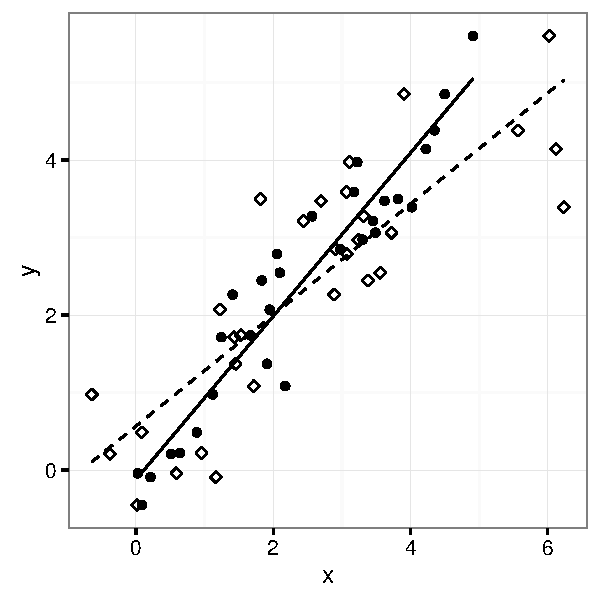
\includegraphics[width=\maxwidth]{figure/classical_lm_ex-1} \caption[Simulated data with observed X (solid dots) and W (diamonds) along with fitted OLS lines]{Simulated data with observed X (solid dots) and W (diamonds) along with fitted OLS lines. Solid is for the true X, and dashed is for the W.}\label{fig:classical_lm_ex}
\end{figure}


\end{knitrout}


% 
% %----------%
% \subsubsection{Linear Regression with Berkson Measurement Error}
% %-----------%
% 
% There are some subtle differences if we are in a case with Berkson Measurement error instead of Classical Measurement error. Recall from (\ref{berkson}) how the Berkson model is set up. Plugging (\ref{berkson}) into (\ref{lm}) we get:
% 
% \begin{align}
% 	\text{{\bf Y}} &= \beta_0 + \beta_1 (\text{{\bf W + U}}) + \epsilon \\
% 	\text{{\bf Y}} &= \beta_0 + \beta_1 \text{{\bf W}} + \epsilon^*
% 	\label{berksonlm}
% \end{align}
% 
% and similar to (\ref{lmbias}) we can check whether the OLS estimate for the Berkson Error Linear Model is unbiased or not:
% 
% \begin{align}
% 	\frac{cov(\text{{\bf Y, W}})}{var(\text{{\bf W}})} &= \beta_1 \frac{\sigma_x^2 -\sigma_u^2}{\sigma_x^2 - \sigma_u^2} = \beta_1
% 	\label{lmberksonbias}
% \end{align}
% 
% So the Berkson model gives an unbiased estimate of the linear relationship between {\bf X} and {\bf Y}, unlike the Classical model. Similarly, the residual variance of this regression is:
% 
% \begin{align}
% 	var(\textbf{Y}|\textbf{W}) = \sigma_e^2 + \beta_1^2 \sigma_x^2 \frac{\sigma_u^2}{\sigma_x^2}
% 	\label{berksonvar}
% \end{align}

% %-------%
% \subsubsection{Correcting for Bias in Linear Model}
% %-------%

From (\ref{lmbias}), one can see the usual OLS estimator for $\beta_1$ using {\bf W} instead of {\bf X} produces a biased estimate for the true relationship between {\bf Y} and {\bf X}. Looking at (\ref{lmbias}), one can note if we knew $\lambda$, then we could get an unbiased estimator of $\beta_1$ by dividing by $\lambda$. Of course we would not expect this to be the case very often. Instead, we could find a consistent estimator for $\lambda$, then divide our estimate of $\beta_1$ by that estimate, and we will have an unbiased estimate for $\beta_1$. Using $\sigma_x^2 = \sigma_w^2 - \sigma_u^2$, we get $\hat{\lambda} = \frac{\hat{\sigma_w^2} - \hat{\sigma_u^2}}{\hat{\sigma_w^2}}$. $\hat{\sigma_w^2}$ and $\hat{\sigma_u^2}$ is the sample variance of the observed {\bf W}'s and the estimated variance of the measurement error, respectively. As long as both of these are consistent (which we know $\hat{\sigma_w^2}$ is), then $\hat{\lambda}$ is consistent for $\lambda$. Carroll et al. gives an estimate for $\sigma_u^2$ on page 71. It turns out in small sample sizes, this estimator for $\lambda$ has a a very skewed distribution, and Fuller \cite{linear} gives a modified version of the above approach to give a more symmetric sampling distribution. The above method is a method of moments estimator because it only depends on moments based on the data and no distributional assumptions are made. 


%--------------------------------%
\subsection{Energy Balance Measurement Error Models}
%--------------------------------%

To the best of our knowledge, no one has attempted to model the energy balance error structure jointly. While there have been measurement error models constructed for both physical activity and various aspects of nutrition, no one has used the joint relationships that exist between physical activity and food consumed (or equivalently physical activity and body composition changes) to assess the measurement error present in today's devices. We will construct our model based on univariate methods developed within the field as well as models constructed with no intent of application in exercise science or nutrition. 


%--------------------------------%
\subsection{Bayesian Measurement Error Models}
%--------------------------------%

Richardson et al. \cite{richardson} presents a general approach to Bayesian modeling of measurement error problems with particular focus on epidemiology applications. This work was done when MCMC methods were becoming popular, and thus this provided a new way to approach these types of problems compared to frequentist methods. The authors propose hierarchical modeling that utilizes conditional independence. The state that the classical measurement error problem can be broken into the three components below: 

\begin{align}
  \text{Disease Model} &= Y_i|X_i,Z_i,\theta_y \\
  \text{Measurement Model} &= W_i|X_i,\theta_w \\
  \text{Exposure Model} &= X_i|Z_i,\theta_x
\end{align}

where $Y_i$ is the response, often representing the presence of a disease. $W_i$ is a surrogate for $X_i$, ie a covariate measured with error. $Z_i$ represent other covariates that are assumed to be error free. The interest in the problem is the influence of the covariates measured with error ($W_i$) and without error ($Z_i$) on the response which is some sort of health outcome, whether it be binary or not. Conditional on the truth covariates $X_i$, $Z_i$, the response is conditionally independent of the surrogate $W_i$. The joint distribution can then be easily written as the product over $i$ of the above model components. Richardson et al. give more details and more complex dependence structures, but this is their general framework. They presented a linear and generalized linear (binomial) measurement error model with normal distributions for errors and exposure, but this general framework can easily be expanded upon.


The paper by Berry et al. \cite{berry02} introduced a fully Bayesian approach to the problem of nonparametric regression when there is measurement error in the covariates. This extends the traditional linear measurement error by allowing a non-linear response of unknown form. They explored the following situation:

\begin{align}
  Y_i &= m(X_i) + \epsilon_i \\
  W_{ij} &= X_i + U_{ij} 
\end{align}

Berry et al. used penalized splines to estimate the function $m()$, and opt to use a relatively large number of knots (20-40). Assuming normal distributions for the error terms as well as the latent variables $X_i$, they present an MCMC algorithm to sample from the posterior. In a simulation study, they showed their model had better frequentist properties than some competeing frequentist methods. They also did some rbobustness checks to their normal assumptions, and although there were some losses of efficiency, the authors note ``the results are at least encouraging in the case of small model deviations". The analysis was also not sensitive to priors. 

Sinha et al. \cite{sinha10} presents a semiparametric Bayesian analysis of nutritional data. In this paper the authors are interested in a binary response variable as unknown function of a variable measured with error plus a linear function of error-free covariates. The authors assume normal errors for the measurement error terms, but place a Dirichlet Process on the latent variables $X_i$ in an attempt to lighten distributional assumptions. The authors used B-splines instead of P-splines and also opted to use a large number of fixed knots. 


Sarkar et al. \cite{sarkar14} presents a semiparametric model that attempts to make as few distributional assumptions as possible. Their setup is nearly identical to Berry et al. They proposed using a Dirichlet Process for the distribution of the latent variables, measurement error, and regression error terms to avoid the standard normality assumption. They also allow for non-constant variance. Sarkar et al. proposes using splines to model the unknown regression function, but they chose to use B-splines largely because they are more stable. The number and location of knots are chosen beforehand. Simulation studies show their model outperforms the model of Berry et al. under various situations. The authors note however, that the model of Berry et al. is competitive when using B-splines instead of the originally proposed P-splines. The authors attributed this to the numerical stability of the B-splines.


%-------------------------------------------------------%
\subsection{Summary}
%-------------------------------------------------------%

In this chapter we motivated the need for reliable, cheap measurements of energy intake.  Many of the methods of measuring energy intake are either heavily biased or very expensive, making either unsuitable for most researchers.   We explained the concept of energy balance and how this principle can be used as an alternative approach to directly measuring EI. The idea of using energy balance has gained popularity in recent years in the field of epidemiology and kinesiology. It is known that measuring EE is easier in terms of cost and convenience compared to EI, and we gave many examples of EE measurement tools. The same is also true with $\Delta$ES. The goal should then be to unify these measurements and share information across them to get a better estimate of EI.


From this, we showed the need for a full measurement error model for energy balance measurements. Measurement error models for energy balance as a whole have not been developed, but the field could benefit greatly from this. Measurement error models would allow researchers to understand how noisy measurements are from certain instruments as well as calibrate biased measurements. This would allow researchers to use the energy balance principle (as many currently are) as a means to measuring EI while accounting for any biases and errors present. Measurement error modeling is well established in statistics, and we reviewed some of the newer, flexible Bayesian methods. These models introduced splines in the regression function and Dirichlet Processes for the latent variables. 

We hope to build upon these models and add a dependence structure that exists in our bivariate framework. 




\bibliographystyle{unsrt} %style of bibliography
\bibliography{references} %tells BibTeX to create a list of references using those in the BibTeX file %research.bib.

\end{document}
